
\chapter{Umsetzung}
\section{Technologien und Tools für Umsetzung } 

\subsection{Java} 
Die drei Teilprojekte der Arbeit wurden in Java entwickelt. Die verwendete Java Version ist Java 11. Java wird als Sprache in der Arbeit verwendet, da eine große Anzahl von Tools für die Statische Code Analyse auf Java passieren und eine plattformunabhängige und robuste Programmiersprache ist. Als Alternative zu Java könnte C-Sharp oder eine JavaScript basierende Webserver-Lösung wie Node.js fungieren.

\subsection{Spring} 
Spring Boot ist ein Java Framework, das im Zuge der Projektarbeit zur Entwicklung der Web-Applikation verwendet wurde.

\subsection{Maven} 
Maven ist ein Versionsverwaltungstool mit dem Abhängigkeiten und JARs verwaltet und heruntergeladen werden können.

\subsection{FindBugs/SpotBugs} 
ERGÄNZEN ERGÄNZEN ERGÄNZEN 

\subsection{Checkstyle} 
Checkstyle ist ein open-source Tool für die Statische Code Analyse. Checkstyle ist für die Verwendung in Java Applikation entwickelt worden. Hierbei werden eine Vielzahl an Fehler und Bugs analysiert und beachtet. Checkstyle kann konfiguriert und an spezifische Probleme angepasst werden

\subsection{MongoDB} 
Als Datenbank wird die nicht-relationale Lösung MongoDB verwendet, da es verschiedene Vorteile gegenüber relationales Datenbankmanagementsystem bietet. (siehe Punkt 4.4.1) Es gehört zu den dokumentorientierten Datenbanken.
MongoDB kann über die offiziele Website heruntergeladen und installiert werden. \cite{mongoDbManual}

\subsection{MongoDB Java Driver}
Der MongoDB Java Driver wird für die Kommunikation (Synchronisation und asynchrone Interaktion) mit MongoDB eingesetzt. Als Alternative kann Jongo (https://jongo.org/) oder  Morphia (https://morphia.dev/) eingesetzt werden. 

\subsection{JavaScript und Frameworks}
Für das Frontend der Webapplikation wird JavaScript eingesetzt. Um zusätzliche Funktionen verwenden zu können, werden folgende JavaScript-Plugins, Frameworks und Libraries verwendet: 
\begin{itemize}
\item \textbf{JQuery} bietet vorgefertigte Funktionen und Animationen die eine vereinfachte Entwicklung gewährleisten. Im Frontend der Arbeit wird JQuery zum Erstellen von Animationen verwendet, wie der Auswahl eines Datums oder das Öffnen eines Tooltips.
\item \textbf{Bootstrap} liefert vorgefertigte Styles, die im Frontend bei Tabellen, Buttons und Texten verwendet werden können.
\item \textbf{DataTables} bietet automatische Pagination und Sortierfunktionen für Tabellen.
\item \textbf{Chart.js} unterstützt das Erstellen von Diagrammen. 
\end{itemize}

\subsection{IntelliJ}
IntelliJ IDEA wurde als Entwicklungsumgebung für das Backend und Frontend verwendet, da es mehrere Programmiersprachen und Frameworks unterstützt.

\section{Infrastruktur und Aufbau der Applikationen} 
Im Rahmen dieser Arbeit wurde mehrere Applikationen und Systeme verwendet. Die Arbeit setzt sich aus folgenden Teilen zusammen:

\begin{figure}[tp]
  \centering
  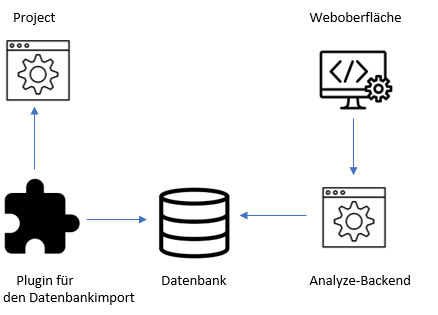
\includegraphics[height=8cm]{images/infrastruktur.PNG}
  % The short caption should be capitalised
  % The full caption should hold a full sentence. 
 \caption[Aufbau der Teilsysteme und Projekte der Arbeit]{Aufbau der Teilsysteme und Projekte der Arbeit.}
  \label{fig:engine}
\end{figure}

Das \textit{Project} ist das Softwareprojekt, welches analysiert werden soll. In diesem Projekt wird auch ein Tool für die Statische Code Analyse eingesetzt. Dieses Tool speichert die Daten (Errors, Warnungen, Informationen) extern. Um diese Daten für die Analyse verwenden zu können, wurde im Rahmen der Arbeit ein \textit{Plugin}, welches das Projekt einsetzten kann, entwickelt. Dieses Plugin greift auf die Daten Statische Code Analyse zu. der Um das Plugin verwenden zu können, muss auch eine \textit{Datenbank} angegeben werden, in welche das Plugin die Daten der Statische Code Analyse des Projekts speichern kann. Die nicht-relationale Datenbank wird auf einem Server gehostet. Um in der Weboberfläche die Daten der Datenbank anzeigen zu können, wird auch ein \textit{Backend} benötigt. Das Backend liest die Daten aus und gibt sie an die Weboberfläche weiter. In der \textit{Weboberfläche} werden die Daten in verschiedenen Diagrammen und Tabellen ausgewertet. Auch ein PDF-Export ist möglich. (siehe Punkt 4.6.2.6 Präsentation der Daten)


\section{Demo-Projekt und Bugreport}
demo projekte allgemein -> unterschiedlichkeit
%https://checkstyle.sourceforge.io/config_filters.html

\subsection{Entwicklungsumgebung Build-in}
eingehen auf verwendete ide und tools; intellij inspection build in 
https://www.jetbrains.com/help/idea/code-inspection.html

\subsection{Maven Plugins}
Viele Tools für die Statische Code Analyse bieten die Möglichkeit, XML-Reports zu genieren. Dies ist möglich mit dem Verwenden der spezifischen Maven-Plugins. ~\parencite{spotBugsUsage} \cite{checkstylePlugin} 
Diese Plugins bieten build-Optionen an, mit dem die XML oder Doc-Reports generiert werden können. Die daraus entstehenden XML-Reports bilden die Datengrundlagen für die Analysen und Visualisierungen im Frontend.
\subsubsection{CheckStyle-Plugin}
Um Checkstyle verwenden zu können, muss das CheckStyle-Plugin nicht verwendet werden. Das Plugin dient zum Export der Daten als XML. Dieses generierte XML bildet den Grundstock für die unterschiedlichen Präsentationen der Daten im Frontend gibt. Um die Daten zu exportieren muss folgender Befehl ausgeführt werden:
\begin{verbatim}
mvn checkstyle:checkstyle
\end{verbatim}
Dieser Befehl muss von der Benutzerin oder dem Benutzer manuell ausgeführt werden. Um den Report automatisch zu erstellen, kann beim Einbinden des Plugin die Phase angegeben werden:

\lstset{
  caption={Das Plugin wird automatisch in der install-Phase ausgeführt.}, 
  basicstyle=\small\ttfamily, 
  label=lst:main, 
  %float=tbhp, % float image to top/bottom/here/page
  language=Java,
  frame=single,
  breaklines=true, % break long source code lines, and add arrow
  postbreak=\mbox{\textcolor{red}{$\hookrightarrow$}\space},
  %  basewidth={0.55em}, 
  % fontadjust}  % adjust these for more appealing appearance
}

% listing with some settings, such as float, for this listing only
\begin{samepage}% with samepage we keep a FLOATing listing on one page
	\begin{lstlisting}[float=tbhp]
<plugin>
  <groupId>org.apache.maven.plugins</groupId>
  <artifactId>maven-checkstyle-plugin</artifactId>
  <version>3.1.1</version>
  <executions>
    <execution>
      <phase>install</phase>
      <goals>
        <goal>checkstyle</goal>
      </goals>
    </execution>
  </executions>
</plugin>
	\end{lstlisting}
\end{samepage}
\subsubsection{SpotBugs-Plugin}
ERGÄNZEN TESTEN
\begin{verbatim}
mvn site
\end{verbatim}
Der Speicherort des generierten XML-Files kann in der Plugin-Konfiguration angegeben werden.


\section{Speichern der Daten} 

Zum Speichern der Daten wird eine Datenbank benötigt. Aufgrund der stark variierenden Daten und da es bei großen Projekten auf einem längeren Zeitraum große Datenmengen an Fehler und Warnungen gefunden werden, wird eine nicht-relationale Datenbank (NoSQL) verwendet. 

\subsection{Vorteil vom Einsatz einer nicht-relationalen Datenbank gegenüber einer relationalen Datenbanke }
Der Vorteil einer nicht-relationalen Datenbank wie MongoDB besteht in der unterschiedlichen Lösung des CAP-Theorem. CAP ist eine für Abkürzung:

\begin{itemize}
\item C = Consistency (Konsistenz)
\item A = Availability (Verfügbarkeit) 
\item P = Partition Tolerance (Fehlertoleranz))
\end{itemize}

Das CAP-Theorem besagt, dass nur zwei dieser Eigenschaften gleichzeitig gelten können. 
Relationale Datenbanken sind im CA Bereich beheimatet, sie legen einen hohen Wert auf Konsistenz. Bei NoSQL und Big Data muss  auf die Fehlertoleranz geachten werden und gleicherweise müssen die Datenbanken hochverfügbar sein, so sind sie im AP Bereich beheimatet. Das garantiert eine hohe Verfügbarkeit und Fehlertoleranz. Konsistenz ist bei den vielen Analysen der Statischen Code Analyse weniger von nutzen, da die Daten der verschiedenen Tools auch stark varrieren. Zusätzlich garantiert die Verwendung einer nicht-relationalen Datenbank eine einfache Query-Language und ein freies Schema.\\
Die Verwendung von nicht-relationalen Datenbanken stellt daher eine Möglichkeit da, die Herausforderungen im Bereich von BigData zu lösen:
\begin{itemize}
\item Größe der Daten (Volume) 
\item Geschwindigkeit der Verarbeitung (Velocity)
\item Strukturierung der Daten (Variety)
\end{itemize}


\subsection{Typen der nicht-relationale Datenbanken}
NoSQL bedeutet nicht \emph{Kein SQL}, sondern \emph{Not only SQL}. Der Aufbau ist hierbei nicht auf relationale Datenbanken beschränkt, sondern kann seine Datenbankstruktur erweitert. 
So gibt es in diesem Umfeld viele Anbieter von NoSQL Lösungen. Diese Lösungen für Datenbanken werden in folgende Kategorien unterteilt:

\begin{itemize}
\item Key Value Datenbanken: Abfragen nur über einen Schlüssel
\item Spaltenorientierte Datenbanken (Dynamische Spalten)
\item Graph-Datenbanken (Verwaltung und Arbeiten mit Knoten)
\item Dokumentorientierte Datenbanken: Besteht aus mehreren Dokumenten (JSONs)
\end{itemize}

Da die Analyseergebnisse der Statischen Code Analyse mehrere Informationen beinhalten, die leicht in JSONs gespeichert werden können, wird die dokumentorientierte Datenbank MongoDB verwendet. 

\subsection{Aufbau der Datenbank}
MongoDB benutzt schemafreie Collections um Daten zu speichern. Schemafreiheit ist nur ein technischer Aspekt. Eine Collection kann Dokumente mit beliebiger Struktur speichern und jedes dieser Dokumente kann sich von den anderen Dokumenten unterscheiden. Trotzdem sollen nicht stark unterschiedliche Dokumente in einer Collection gespeichert werden, da es in der Verwaltung bei einer starken Abweichung einen großen zusätzlichen Aufwand gibt. 

Für die Analyseergbnisse wird eine Collection verwendet, die folgende Felder beinhalten kann: \textit{id, project, file, line, message, source, severity, date}

Beispiel eines JSON-Datensatzs in der Collection:

\begin{verbatim}
{ "_id" : ObjectId("5e1209881a2dff20ab6ee6c6"), 
"project" : "importerProject", 
"file" : "Sender.java", 
"line" : 72, 
"message" : "Not closed!", 
"source" : "checkstyle.checks.blocks.AvoidNestedBlocksCheck", 
"severity" : "error", 
"date" : ISODate("2020-01-05T00:00:00Z") }
\end{verbatim}

In einer relationalen Datenbanken mit einem starken Schema und einer ausgeprägten Konsistenz, könnte dieser Datensatz in mehrere Tabellen verteilt gespeichert werden, zum Beispiel eine eigene Tabelle für \textit{severity}. Aufgrund der schwachen Konsistenz in nicht-relationalen Datenbanken wird hierbei nur eine Collection (Tabelle) verwendet. So können in dieser Collection auch Datensätze gespeichert werden, die keine \textit{severity} besitzen: NULL-Werte können so nicht auftreten. \\
Die Datensätze können mit dem Mongo-Service ausgelesen werden: 

\begin{verbatim}
// Lesen aller Daten:
db.findings.find({})

// Lesen eines bestimmten Datensatzes:
db.findings.find({"_id" : ObjectId("5e1209881a2dff20ab6ee6c6")})
\end{verbatim}

Eine zweite Collection \textit{recommendations} wird für das Speichern der Vorschläge für die Fehler und Warnungen verwendet. Benutzer können hierbei über die Webapplikation Tutorials und nützliche Links zu den einzelnen Fehlern und Warnungen speichern.
In dieser Collection werden daher Objekte mit nur zwei Datenfeldern gespeichert: \textit{error} und \textit{link}. \\
In einer dritten Collection \textit{ignoredFindings} werden Errors und Warnungen gespeichert, die von der Anzeige im Frontend ausgenommen werden. In den Objekten gibt es nur ein Datenfeld \textit{message}, für die ausgenommen Meldungen.
\section{Datenbank Importer Plugin} 
Die Statischen Code Analyse wird auf dem Rechner des Entwicklers oder der Entwicklerin ausgeführt. Diese Daten müssen in der Datenbank gespeichert werden, um sie in einem längeren Zeitraum einsehen und auswerten zu können. Eine eigene Lösung wird daher benötigt, um die Daten in der Datenbank speichern zu können. 
\subsection{Apache Maven Plugin}
Mit Apache Maven können verschiedene Plugins eingebunden und im Projekt verwendet werden. Apache Maven bietet aber auch die Möglichkeit, eigene Plugins zu entwickeln.\cite{anardu2014maven}

Die Dependency \textit{maven-plugin-api} gibt Klassen und Funktionen vor, die benutzt werden können um ein eigenes Plugin zu entwickeln
\begin{verbatim}
 <dependency>
      <groupId>org.apache.maven</groupId>
      <artifactId>maven-plugin-api</artifactId>
      <version>3.6.0</version>
      <scope>provided</scope>
 </dependency>
\end{verbatim}

Mit dieser Dependency kann nun eine Mojo-Klasse erstellt (siehe Listing  \ref{lst:mainexecuter}). Die Klasse \textit{MainExecuter.java} stellt den Kern des Plugins da, die der Verwendung des Plugins zuerst ausgeführt wird.  \cite{gonzalezMavenTutorial}

\lstset{
  caption={Kopf der Executor-Klasse: Sie wird mit dem Aufruf des Plugins zuerst gestartet.}, 
  basicstyle=\small\ttfamily, 
  label=lst:mainexecuter, 
  %float=tbhp, % float image to top/bottom/here/page
  language=Java,
  frame=single,
  breaklines=true, % break long source code lines, and add arrow
  postbreak=\mbox{\textcolor{red}{$\hookrightarrow$}\space},
  %  basewidth={0.55em}, 
  % fontadjust}  % adjust these for more appealing appearance
}

% listing with some settings, such as float, for this listing only
\begin{samepage}% with samepage we keep a FLOATing listing on one page
	\begin{lstlisting}[float=tbhp]
@Mojo(name = "import", defaultPhase = LifecyclePhase.INSTALL)
public class MainExecutor extends AbstractMojo {

    @Parameter(property = "dbName",defaultValue = "findings")
    private String dbName;
	\end{lstlisting}
\end{samepage}
	

Um die Klasse \textit{MainExecuter.java} als Mojo-Klasse zu kennzeichen, muss von \textit{AbstractMojo} abgeleitet und mit \textit{@Mojo} annotiert werden.

%\includegraphics{/dbpluginConnect.PNG}

Mit der Option \textit{defaultPhase} kann festgelegt werden, in welcher Maven-Lifecycle-Phase das Plugin ausgeführt werden soll. Mit dieser Einstellung wird das Plugin während des install-Prozesses ausgeführt. Weitere Möglichkeiten sind unter anderen die Phasen  \textit{deploy},  \textit{clean} und  \textit{compile}. \\

Das Plugin wird mit bestimmten Parametern aufgerufen. Diese können beim Einbinden des Plugins angegeben werden. Folgende Parameter werden benötigt, um das Plugin auszuführen:

\begin{itemize}
\item \textit{dbName}: Name der Datenbank, indem die Ergebnisse der Statischen Code Analyse gespeichert werden. 
\item \textit{dbUrl}: URL für die Datenbank
\item \textit{xmlFile}: Name des generierten XML-Files
\end{itemize}
  
% \includegraphics{dbpluginParameter}    

In der Mojo-Klasse muss die Methode \textit{execute} implementiert werden, die zu Beginn, beim Start des Plugins, ausgeführt wird. Mithilfe der oben definierten Parameter und des Projektnamens, der mit dem Maven-Lifecycle ausgelesen werden kann, wird nun der Import in die Datenbank gestartet. 

\subsection{MongoDB-Java-Driver und Datenbank-Import}
Der Importer speichert die Daten des XML-Reports in Datenbanken. Dazu wird das XML-File ausgelesen und die einzelnen gefundenen Fehler und Informationen werden in Java-Objekte umgewandelt. Das Speichern der Java-Objekte in den Collections ist ohne Konvertierung, im Vergleich zu anderen herkömmlichen Tools wie Hibernate, nicht möglich. Um Daten zu speichern, müssen die Java-Objekte in Dokumente umgewandelt werden. Daher muss ein Konverter implementiert werden: \textit{DBObjectConverter}
Bei steigender Komplexität und Größe der Datenbank können die Konverter sehr komplex werden. Der Typ \textit{org.bson.Document} wird vom MongoDB-Java-Driver vorgegeben. Ein BSON-Dokument unterscheidet sich nur von der Kodierung zu Json-Objekte. (BSON=Binary Json) 
Diese Dokumente können nun für die Datenbank-Transaktionen verwendet werden. Bei steigender Komplexität und Größe der Datenbank werden auch die Konverter komplexer, da alle Felder, Datentypen und Object-Arrays beachtet werden müssen.
 \\

Um die Dokumente speichern zu können, muss eine Verbindung zur Datenbank mit den eingegebenen Parametern erstellt werden. Dazu müssen Objekte mit den Typen \textit{MongoClient}, \textit{MongoDatabase} und \textit{MongoCollection} initialisiert und verwendet werden (siehe Listing \ref{lst:mongoAtr}).

\lstset{
  caption={Benötigte Attribute, um sich mit der Datenbank verbinden und die Collections verwenden.}, 
  basicstyle=\small\ttfamily, 
  label=lst:mongoAtr, 
  %float=tbhp, % float image to top/bottom/here/page
  language=Java,
  frame=single,
  breaklines=true, % break long source code lines, and add arrow
  postbreak=\mbox{\textcolor{red}{$\hookrightarrow$}\space},
  %  basewidth={0.55em}, 
  % fontadjust}  % adjust these for more appealing appearance
}

% listing with some settings, such as float, for this listing only
\begin{samepage}% with samepage we keep a FLOATing listing on one page
	\begin{lstlisting}[float=tbhp]
	
mongoClient = new MongoClient(new MongoClientURI(dbUrl));
db = mongoClient.getDatabase(databaseName);
db = mongoClient.getDatabase(databaseName);

	\end{lstlisting}
\end{samepage}

Der Typ \textit{MongoCollection<Document>} kann nun verwendet werden um Dokumente zu speichern, löschen oder auszulesen. Diese Operationen werden beim MongoDB-Java-Driver direkt auf die betreffenden Collections angewendet. Ein Commit oder eine andere Operation ist dabei nicht notwendig.

% \includegraphics{dbpluginSave}    

\section{Webapplikation} 
Die Webapplikation bildet den zentralen Teil der Applikation. Das Ziel ist es, die gespeicherten Daten für die Benutzerinnen und Benutzer übersichtlich und einfach aufzubereiten. 
\subsection{Backend}
Im Backend werden die Daten aus der Datenbank in Services ausgelesen. Die ausgelesen Daten werden in Beans umgewandelt. Über die REST-Schnittstelle können Daten an das Frontend übergeben werden. Das Backend bzw. die Webapplikation verwendet das Framework Spring-Boot als Alternative zu Java EE. ~\parencite{walls2016spring} Spring Boot bietet einen Standalone-Server und kann daher ohne Konfigurationen verwendet werden. Zusätzlich bietet Spring Boot die Möglichkeit zur Erstellung von Spring Beans und REST-Controller.  

\subsubsection{Struktur}
aufbau der packages und files; image
\subsubsection{API und Controller}
Über den Controller können HTTP-Requests an das Backend geschickt werden. Mit Spring können die Controller als \textit{RestController} annotiert und verwendet werden. Die einzelnen Methoden des Controllers werden zusätzlich annotiert um die Methode (GET, POST, DELETE, PUT, ...) und den Pfad zu definieren. Im Pfad können zusätzlich Parameter als \textit{PathVariable} definiert werden. Im Controller werden  Methoden verwendet um bestimmte Projektanalysedaten auszulesen, Daten als PDF zu exportieren und um Vorschläge zu speichern und auszulesen. Im \textit{FindingsController} werden die Anfragen aus dem Frontend bearbeitet und Daten an des Frontend übermittelt. Im Controller sind dazu die verschiedenen Services eingebunden.
\subsubsection{Services und MongoDB-Java-Driver}
In den Services werden Methoden bereitgestellt, die die Daten der Datenbank auslesen. Dies geschieht mit dem MongoDB-Java-Driver. Für das Verwenden des MongoDB-Java-Driver ist ein spezifischer Converter notwendig. Wie im Importer-Plugin müssen die Daten konvertiert werden, daher wird ein Konverter \textit{DBObjectConverter.java} auch im Backend verwendet.
\lstset{
  caption={Um die Datenbank benutzen können, müssen die Java-Objekte bzw. die Datenbank-JSON-Objekte konvertiert werden.}, 
  basicstyle=\small\ttfamily, 
  label=lst:main, 
  %float=tbhp, % float image to top/bottom/here/page
  language=Java,
  frame=single,
  breaklines=true, % break long source code lines, and add arrow
  postbreak=\mbox{\textcolor{red}{$\hookrightarrow$}\space},
  %  basewidth={0.55em}, 
  % fontadjust}  % adjust these for more appealing appearance
}

% listing with some settings, such as float, for this listing only
\begin{samepage}% with samepage we keep a FLOATing listing on one page
	\begin{lstlisting}[float=tbhp]
public static Finding convertToObject(Document e) {
    String project = (String) e.get("project");
    String file = (String) e.get("file");    
    ...

public static Document convertToDocument(Recommendation rec) {
    org.bson.Document recDoc = new Document();
    recDoc.append("error", rec.getError());
    recDoc.append("link", rec.getLink());
    ...
	\end{lstlisting}
\end{samepage}

Der Konverter wird in allen Service-Methoden verwendet, wo Daten aus den Collections mit dem MongoDB-Java-Driver ausgelesen, gespeichert oder gelöscht werden. Um diese Operation zu verwenden, müssen die Methoden \textit{find}, \textit{deleteOne} und \textit{insertOne} verwendet werden. Um bestimmte Daten auszuwählen, wird in der Methode \textit{find} ein Query-Parameter übergeben: In den entsprechenden Services ein Projektname oder ein Datum. Die Ergebnisse werden mit einem Iterator iteriert und an den Konverter übergeben. Eigene Services gibt es für alle Datenbank Collections: Findings, Recommendation, IgnoredMessages.

\subsubsection{IText und PDF-Export}
Der PDF-Export ist eine weitere Funktion, die das Backend bietet. Ein PDF-Export kann für ein bestimmtes Projekt in einem bestimmten Zeitraum erstellt werden. Im Report werden die wichtigsten Informationen der Analyse in Textform dargestellt, dazu auch die einzelnen gefundenen Fehler und Warnungen. \\
Dazu wird das Tool IText zur Erstellung von Reports verwendet.  \cite{lowagie2011itext} Um IText zu verwenden, kann aus verschiedenen Preismodellen gewählt werden, eine kostenlose Version wird aber auch zur Verfügung gestellt und in dieser Arbeit verwendet.  \\
Über das Service liest der PDF-Generator die angegeben Daten aus.

\lstset{
  caption={Initialisierung des Writers um im Dokument einen Paragraph zu erstellen.}, 
  basicstyle=\small\ttfamily, 
  label=lst:main, 
  %float=tbhp, % float image to top/bottom/here/page
  language=Java,
  frame=single,
  breaklines=true, % break long source code lines, and add arrow
  postbreak=\mbox{\textcolor{red}{$\hookrightarrow$}\space},
  %  basewidth={0.55em}, 
  % fontadjust}  % adjust these for more appealing appearance
}

% listing with some settings, such as float, for this listing only
\begin{samepage}% with samepage we keep a FLOATing listing on one page
	\begin{lstlisting}[float=tbhp]
PdfWriter writer = PdfWriter.getInstance(
   document, byteArrayOutputStream);
document.open();
document.add(new Paragraph(
  "Findings PDF Export. - " +LocalDate.now(), titleFont));

	\end{lstlisting}
\end{samepage}

Für alle im Service ausgelesen Daten wird ein eigener Paragraph erstellt. Um die Überschrift und die Daten entsprechend zu formatieren, kann mittels \textit{IText} auch ein Font erstellt werden. Mit der \textit{FontFactory} wird hierbei ein Font mit bestimmter Schriftart, Schriftgröße und Farbe erstellt.
Nach der Erstellung des PDF-Dokument muss das Ergebnis weiter an den Client geschickt werden. Um das PDF-Dokumente im \textit{Response} der HTTP-Anfrage zu übertragen, wird das Dokument in ein \textit{byte-array} konvertiert. Dies geschieht mit der Verwendung des \textit{ByteArrayOutputStream} und dessen Methode \textit{toByteArray}. 

\begin{figure}[tp]
  \centering
  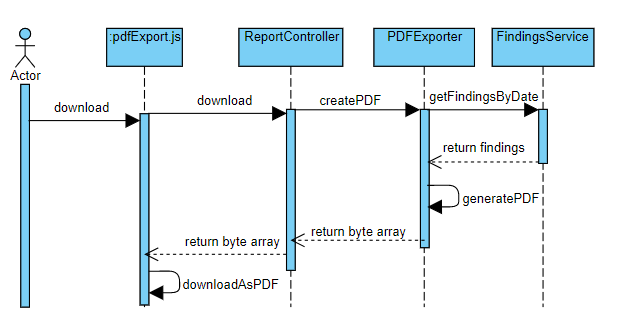
\includegraphics[height=8cm]{images/seqGeneratePdf.PNG}
  % The short caption should be capitalised
  % The full caption should hold a full sentence. 
 \caption[Sequenzdiagramm für den Download eines PDF-Exports]{Sequenzdiagramm für den Download eines PDF-Exports.}
  \label{fig:engine}
\end{figure}

\subsection{Frontend}
Im Frontend werden die Daten in verschiedenen Formen aufbereitet und den Entwicklerinnen und Entwicklern präsentiert, dazu dient eine OnePage-HTML Seite. Die Daten im Frontend werden aus dem Backend abgefragt.
\subsubsection{Struktur}
aufbau der ordner und files; image
\subsubsection{Kommunikation mit dem Backend}
Die Kommunikation zwischen Frontend und Backend geschieht mittels HTTP-Calls. Die im Frontend gesendeten HTTP-Calls werden im Backend-Controller verarbeitet.  Mit der JavaScript Schnittstelle \textit{Fetch API} werden HTTP-Methoden (POST, GET) abgeschickt. Ein Vorteil der  \textit{Fetch API} ist die Möglichkeit der asynchronen Ausführung der Requests. Daher können auch dynamische Daten abgerufen werden. \footnote{https://developers.google.com/web/updates/2015/03/introduction-to-fetch}
\lstset{
  caption={Erstellung eines GET-Request für Projektdaten mit der Schnittstelle Fetch API.}, 
  basicstyle=\small\ttfamily, 
  label=lst:fetchApiGet, 
  %float=tbhp, % float image to top/bottom/here/page
  language=Java,
  frame=single,
  breaklines=true, % break long source code lines, and add arrow
  postbreak=\mbox{\textcolor{red}{$\hookrightarrow$}\space},
  %  basewidth={0.55em}, 
  % fontadjust}  % adjust these for more appealing appearance
}

% listing with some settings, such as float, for this listing only
\begin{samepage}% with samepage we keep a FLOATing listing on one page
	\begin{lstlisting}[float=tbhp]
fetch(urlProjects)
  .then(function(response) {
     return response.json();
   })
  .then(function(json) {
     var result = json;
        
  	 result.forEach(function (entry) {
        var opt = document
           .createElement('option');
        var projectname = entry;
        opt.value = projectname;
        opt.id = projectname;
        opt.innerHTML = projectname;
            projectData.appendChild(opt);
        });
        
    }).catch(function (error) {
        console.log('Failure: ', error);
    });

	\end{lstlisting}
\end{samepage}

Im Listing werden allgemeine Daten der Projekte abgefragt (siehe Listing \ref{lst:fetchApiGet}). Da bei der Abfrage keine Daten am Server verändert werden, wird ein GET-Requests erstellt. Ist die Abfrage erfolgreich, so werden die einzelnen \textit{then}-Blöcke ausgeführt. Im ersten Block werden die Daten des Response zu JSON-Objekte konvertiert. Um die Daten verwenden zu können, werden die einzelnen JSON-Objekte in einem Result-Array gespeichert.  \\
Im Gegensatz zum GET-Request steht der POST-Request. Hierbei werden Daten an den Server übermittelt. Im Frontend werden diese Anfragen für das Erstellen von Recommendations und zum Ignorieren von Meldungen verwendetet. Um einen POST-Request zu erstellen, müssen die Attribute \textit{param} und \textit{method: 'POST'} angegeben werden. Die Daten können mittels dem Attribut \textit{param} übergeben werden. \\
Treten beim Request Fehler auf, so werden die Anweisungen im \textit{catch}-Block ausgeführt.

\subsubsection{Recommendations}
In der Weboberfläche können gezielt Vorschläge (Recommendations) für einzelne Fehlermeldungen und Warnungen hinterlegt werden. Um eine Recommendation zu erstellen, muss in der Weboberfläche in der Recommendations-Section ein neuer Eintrag mit einer Fehlermeldung und einem Link auf eine Lösung hinterlegt werden. Diese Lösungen können beispielsweise Tutorials, Dokumentationen oder andere gezielte Hilfsstellungen für die Meldung sein. Diese Recommendations werden in der Datenbank gespeichert.

Um zur einer bestimmte Meldung einen Link zu speichern, muss nicht die ganze Meldung gespeichert werden. Es kann auch nur ein Teil aus der Meldung gespeichert werden. Diese Funktionalität unterstützt so auch das Erstellen von Recommendations für spezifische Meldungen:

\textit{Die Variable 'name' verbirgt ein Feld.}\\
\textit{Die Variable 'artist' verbirgt ein Feld.}

Wird in diesem Beispiel die Meldung \textit{verbirgt ein Feld} als Recommendation gespeichert, so erscheint die Recommendation für alle Meldungen (siehe Abbildung \ref{fig:recommendations}), die diesen Text in der Beschreibung beinhalten, der Variablenname kann so ignoriert werden. 

\begin{figure}[tp]
  \centering
  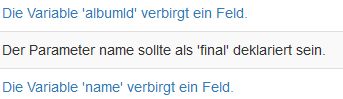
\includegraphics[height=2cm]{images/recommendation.PNG}
  % The short caption should be capitalised
  % The full caption should hold a full sentence. 
 \caption[Anzeige der Meldung mit dem hinterlegten Recommendation-Link. Der Link führt in diesem Beispiel zur genauen Beschreibung des Fehlers in einer Dokumentation]{Anzeige der Meldung mit dem hinterlegten Recommendation-Link. Der Link führt in diesem Beispiel zur genauen Beschreibung des Fehlers in einer Dokumentation}
  \label{fig:recommendations}
\end{figure}

\subsubsection{Ignorieren von Meldungen}
Die Analyseergebnisse der Tools für die Statische Code Analyse beinhalten auch Bugs und Informationen, die für Entwicklerinnen und Entwickler irrelevant, überflüssig  oder aus anderen Gründen nicht beachtet werden sollen. Die Weboberfläche bietet daher die Möglichkeit an, bestimmte Meldungen zu ignorieren. Wird eine Meldung von der Benutzerin oder dem Benutzer ignoriert, so scheint sie nicht in der Übersichtstabelle auf und wird auch in den Visualisierungen nicht beachtet. 

Um eine Meldung zu ignorieren, muss der Text einer Meldung in der \textit{Ignore-Table} gespeichert werden. Wie beim Speichern von Recommendations, ist es nicht notwendig den ganzen Text der Meldung zu speichern, es kann auch nur ein Teil der Meldung angegeben werden.  
Die Meldung wird in der Datenbank gespeichert und im Backend aus den Abfrageergebnissen gefiltert. Alle ignorierten Meldungen können in der \textit{Ignore-Table} eingesehen werden (siehe Abbildung \ref{fig:ignoredMessages}). Hier kann auch ein Bug aus der Tabelle gelöscht werden, um wieder in den Visualisierungen und in der Übersichtstabelle eingebunden zu werden.

\begin{figure}[tp]
  \centering
  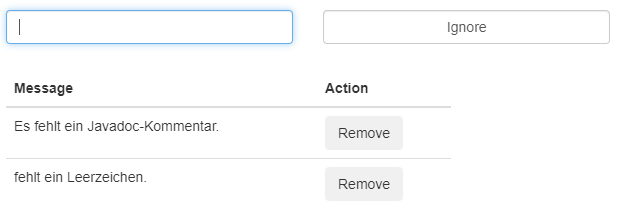
\includegraphics[height=4cm]{images/ignoreTable.PNG}
  % The short caption should be capitalised
  % The full caption should hold a full sentence. 
 \caption[Übersichtstabelle mit ignorierten Meldungen. Diese Meldungen, oder Meldungen die diese Texte beinhaltet, werden ignoriert. Die Meldungen können aus der Ignore-Table gelöscht und im oberen Textfeld gespeichert werden.]{Übersichtstabelle mit ignorierten Meldungen. Diese Meldungen, oder Meldungen die diese Texte beinhaltet, werden ignoriert. Die Meldungen können aus der Ignore-Table gelöscht und im oberen Textfeld gespeichert werden}
  \label{fig:ignoredMessages}
\end{figure}

\subsubsection*{Algorithmus}
Um die ignorierten Meldung zu filtern, müssen alle Meldungen mit allen ignorierten Meldungen verglichen werden. Um die Meldungen zu filtern ergibt sich daher ein Algorithmus mit der Laufzeit \textit{O(n)}. Wird die Anzahl an ignorierten Meldungen aber erhöht, so erhöht sich auch die Laufzeit des Algorithmus stark. Bei der Erstellung der Recommendations wird der gleiche Algorithmus verwendet.

\subsubsection{Erstellen von Grafiken}
Ein zentraler Bestandteil des Frontends sind die Visualisierungen. Hierbei werden die Fehler und Bugs in verschiedenen Grafiken aufbereitet. Um Grafiken(Charts) zu erstellen, wird die open-source Library Chart.js verwendet. Chart.js unterstützt das Erstellen von verschiedenen Grafiktypen wie Balken, Linien, Kreis oder Netzdiagramme. ~\parencite{chartJsHelder} Um eine Grafik mit Chart.js erstellen zu können, werden zwei Datenquellen benötigt: Ein Datenset für die Datenquelle und ein weiteres Set für die dazugehörigen Labels. Diese zwei Sets müssen von gleicher Länge sein, da die Zuordnung der Datenquellen mit den Labels stellenweise erfolgt (siehe Abbildung \ref{lst:pieChart}).

\lstset{
  caption={Erstellen eines Kreisdiagramms mit Chart.js.}, 
  basicstyle=\small\ttfamily, 
  label=lst:pieChart, 
  %float=tbhp, % float image to top/bottom/here/page
  language=Java,
  frame=single,
  breaklines=true, % break long source code lines, and add arrow
  postbreak=\mbox{\textcolor{red}{$\hookrightarrow$}\space},
  %  basewidth={0.55em}, 
  % fontadjust}  % adjust these for more appealing appearance
}

% listing with some settings, such as float, for this listing only
\begin{samepage}% with samepage we keep a FLOATing listing on one page
	\begin{lstlisting}[float=tbhp]
var projectPieChart = new Chart(
document.getElementById("pieChartProjects"), {
   type: 'pie',
    data: {
       labels: pieData[0],
       datasets: [{
          label: "findings",
          backgroundColor: colors,
          data: pieData[1]
       }]
    },
    options: {
       title: {
          display: true,
            text: 'Findings per project'
       }
    }
});
	\end{lstlisting}
\end{samepage}

Bei der Konfiguration des Charts können auch mehrere Attribute angegeben werden, wie der Diagrammtyp, der angezeigte Text der Legende oder die verwendeten Farben. 

Bei der Erstellung eines Balken-Diagramms muss der Typ \textit{horizontalBar} gesetzt werden. Weitere Konfigurationsmöglichkeiten bei Balkendiagrammen sind Werte wie die Größe der Balken (barThickness), der Startwert der Achsen (beginAtZero) oder das Stapeln der Balken. (stack)

Um die erstellten Charts wieder zu löschen und bei neuen Requests neu erstellen zu können müssen die Charts mit der Funktion \textit{destroy} gelöscht werden, auch damit die Referenzen und Cache-Daten verworfen werden können. \footnote{https://www.chartjs.org/docs} Dazu werden die Charts im globalen JavaScript-Objekt \textit{window} gespeichert und wieder entfernt. 

\subsubsection{Präsentation der Daten}
\textbf{Übersichtstabelle} \\
\textbf{Verteilung auf Projektebene} \\
\textbf{Verteilung auf Packageebene} \\
\textbf{Am häufigsten vorkommende Fehler} \\
\textbf{Klassen mit den meisten Problemen} \\
\textbf{Export der Daten als PDF} \\
Eine weitere Möglichkeit im Frontend die Daten anzeigen zu können, ist der PDF-Report. Der Report verwendet dabei die gleichen Daten, die für die anderen Darstellungen ausgewählt wurden. Der Report kann in über einen Download-Button heruntergeladen werden. Erstellt wird der Report im Backend (siehe 4.6.1.4). Um den Report erstellen zu können, wird ein Request versendet, der Report wird daraufhin am Backend generiert und an das Frontend zurückgegeben. Um im Frontend das PDF herunterladen zu können, wird die Blob-Funktionalität verwendet. \footnote{https://developer.mozilla.org/de/docs/Web/API/Blob}

\lstset{
  caption={Herunterladen eines PDF-Files in Javascript mit Blob.}, 
  basicstyle=\small\ttfamily, 
  label=lst:blobDownload, 
  %float=tbhp, % float image to top/bottom/here/page
  language=Java,
  frame=single,
  breaklines=true, % break long source code lines, and add arrow
  postbreak=\mbox{\textcolor{red}{$\hookrightarrow$}\space},
  %  basewidth={0.55em}, 
  % fontadjust}  % adjust these for more appealing appearance
}

% listing with some settings, such as float, for this listing only
\begin{samepage}% with samepage we keep a FLOATing listing on one page
	\begin{lstlisting}[float=tbhp]
.then(function(response) {
   return response.blob(); 
})
.then(function (blobObj) {
   var objectUrl = URL.createObjectURL(blobObj);
   var a = document.createElement('a');
   a.href = objectUrl;
   a.download = project + "Report.pdf";
   document.body.appendChild(a);
   a.click();
   a.remove(); 
})
.catch(function (error) {
   console.log('Request failure: ', error);
});
	\end{lstlisting}
\end{samepage}

Blob(Binary Large Object) bietet die Möglichkeit Dateien zu speichern. Zusätzlich zu Dateidaten speichert Blob einen MIME-Type. Mit dem MIME-Type (Media Type) kann die Art der Daten angegeben werden, in diesem Beispiel hat der MIME-Type den Wert \textit{application/pdf}. Hierbei wird der Reponse bei einem erfolgreichen Request zu einem blob-Objekt konvertiert. Um einen Download durchführen zu können, wird ein Url-Objekt und ein Link erstellt. Der Link wird automatisch geklickt und es erfolgt der Download. Der Hilf-Link wird nach dem Download wieder gelöscht.

\subsection{Vergleiche mit herkömmlichen Lösungen} 
hinsichtlich der Linienmarkierung in Entwicklungsumgebungen
vergleichen auch mit SpotBugs GUI
mehrere Entwickler verfälschen ergebnis
viele analyse tools Vielfalt
\section{Evaluierung der Visualisierung und der Webapplikation} 